% !TeX root = main.tex
% =========================================================================
% REBUTTAL FIGURES (round 2): one \newcommand per figure, typeset with [H]
% and the caption placed outside the float with \captionof{figure}{...},
% same pattern as ../rebuttal/figures.tex. Example:
%
% \newcommand{\figExample}{%
% \begin{figure}[H]
%   \centering
%   \includegraphics[width=\linewidth,height=0.95\textheight,keepaspectratio]{figures/FIGURE_example.pdf}
% \end{figure}
%
% \captionof{figure}{\textbf{Title.} \textbf{(A)} ...}
% \label{fig:example}
% }
% =========================================================================

% ------------------------------------------------------------------ R2.3b
\newcommand{\figRampFish}{%
\begin{figure}[H]
  \centering
  \begin{minipage}{\linewidth}
  \centering
  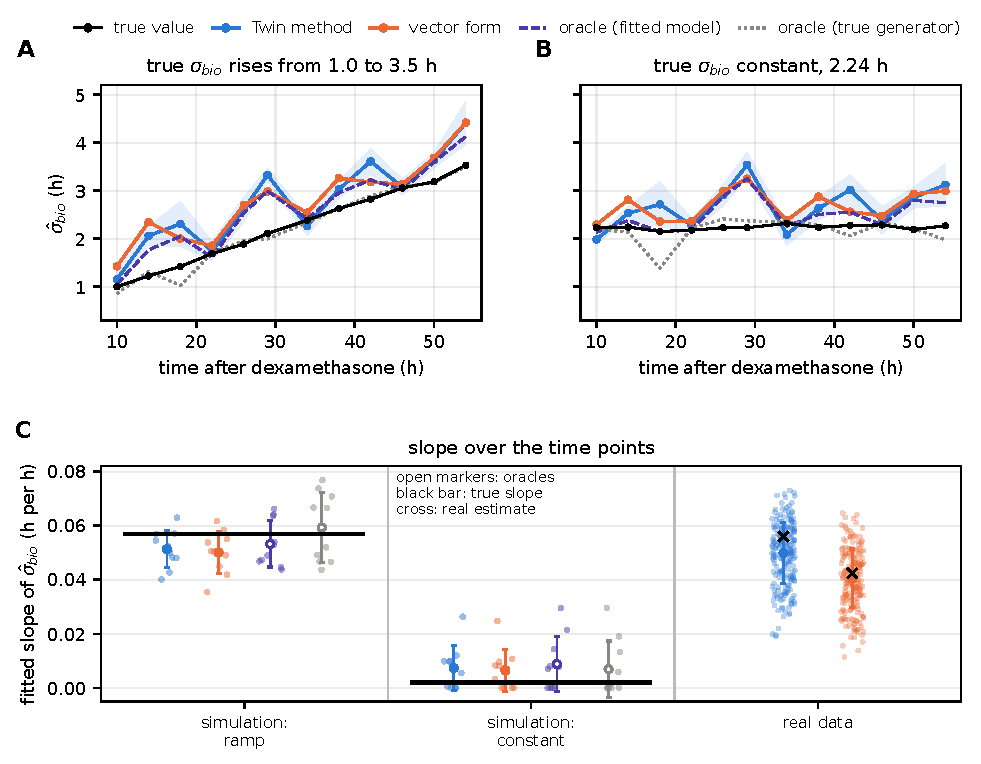
\includegraphics[width=0.9\linewidth,height=0.47\textheight,keepaspectratio]{figures/FIGURE_ramp_fish.pdf}

  {\footnotesize
  \captionof{figure}{\textbf{A simulated copy of the SABER-FISH experiment, with a known $\sigma_{\text{bio}}$ at each time point, next to the real data.}
  \textbf{(A, B)} The estimates follow a rising true $\sigma_{\text{bio}}$ but sit above it. Simulation from the fitted model of the real data (4 genes), with the 12 time points and the numbers of cells of the real experiment and the cell areas of the real cells of each time point as library sizes. The model was fitted again on each of the 10 simulated datasets, and the estimates were made with the same settings as for the real data. Estimated $\sigma_{\text{bio}}$ at each time point when the true value rises from 1.0 to 3.5 h (A) and when it is constant at 2.24 h (B). Black: true value, the circular standard deviation of the true phases of the simulated cells of that time point, so it varies a little around the design value. Blue and orange: Twin method and vector form, mean over the replicates. Blue band: standard deviation of the Twin method over the replicates (the band of the vector form is similar). Dashed purple: oracle with the fitted model, which knows the true phase of every cell and simulates the time point again with the fitted model. Dotted grey: the same oracle with the model that generated the data. The time point at 18 h has the fewest cells (116).
  \textbf{(C)} The slope is recovered in simulation, and it is smaller and less certain in the real data. Slope of the line fitted to the estimates of the 11 time points after the first one, as for the real data (the slope is not allowed to be negative). Same colors as in A. The two oracles have open markers (fitted model in purple, true generator in grey). Black bar: slope of the same line fitted to the true values. Small dots: the 10 replicates for the simulations, and 50 bootstrap draws over the cells for the real data (the model is not fitted again in the bootstrap, so the spread of the dots is smaller than it would be with a new fit). Large markers: mean and standard deviation of the dots. Cross: slope of the real estimates without the bootstrap.
  \textbf{(D)} The real estimates scatter more than the simulated ones. Real data, 116 to 362 cells per time point. Twin method and vector form with the 95\% bootstrap interval over the cells (points are shifted sideways by 0.5 h for legibility). At 18 h the observed spread is smaller than the technical spread, and the Twin estimate is set to zero.}
  \label{fig:ramp_fish}
  }
  \end{minipage}
\end{figure}
}

% ------------------------------------------------------------------ R2.3c
\newcommand{\figRampRnaseq}{%
\begin{figure}[H]
  \centering
  \begin{minipage}{\linewidth}
  \centering
  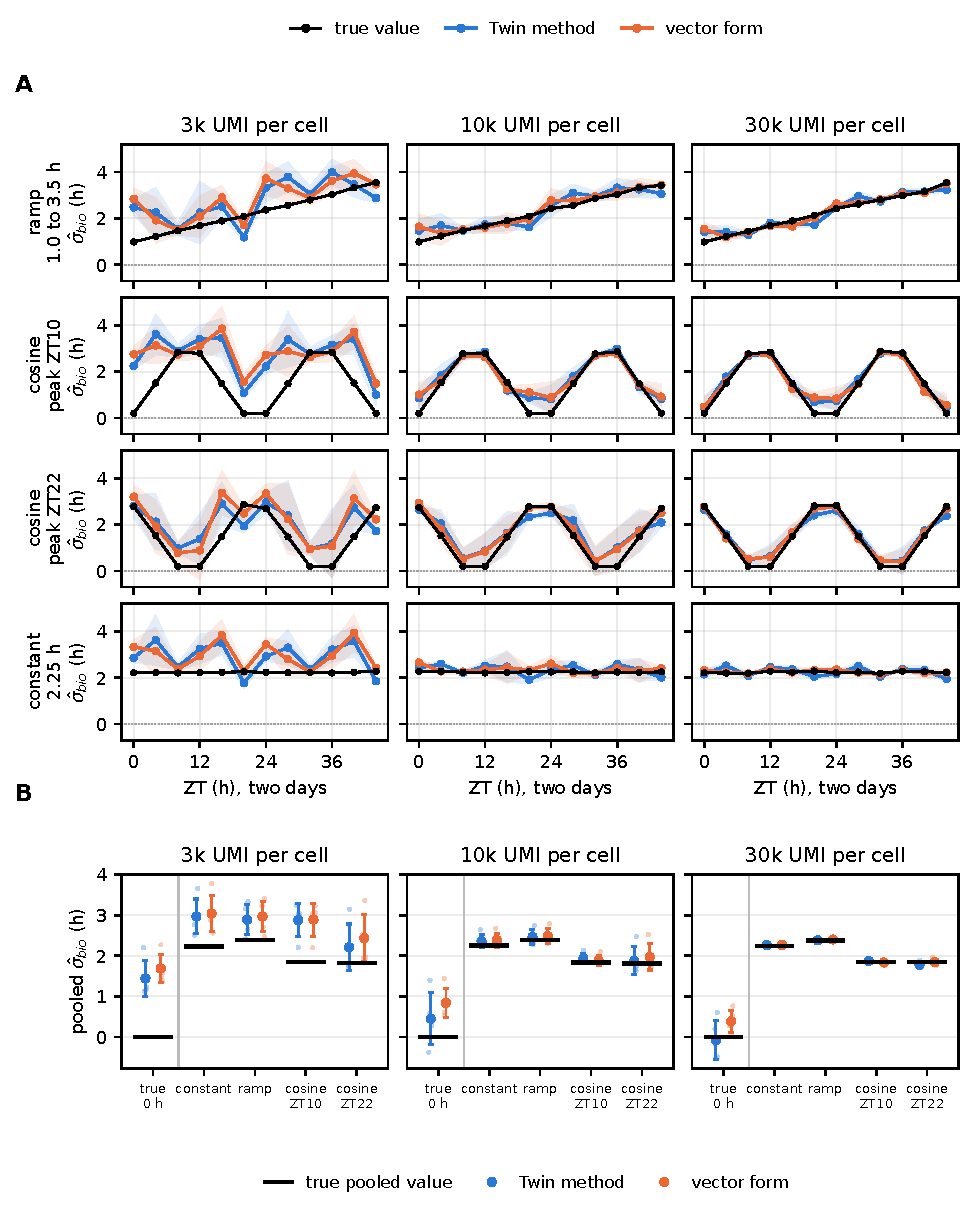
\includegraphics[width=\linewidth,height=0.72\textheight,keepaspectratio]{figures/FIGURE_ramp_rnaseq.pdf}

  {\small
  \captionof{figure}{\textbf{Simulations with a $\sigma_{\text{bio}}$ that changes across time points.}
  15 clock genes, 12 time points over two days, 500 cells per time point, 5 replicates per setting. Columns are the depths.
  \textbf{(A)} Estimated $\sigma_{\text{bio}}$ at each time point for four true profiles (rows). Black: true value. Lines: mean over the replicates. Bands: standard deviation over the replicates. The true cosine is sampled every 4 h (0.2 to 2.8 h) and repeats on the second day.
  \textbf{(B)} The single value over all time points (\maineq{16}) for the same profiles (cosine ZT10 and ZT22 are the two cosines of A) and for a control with a true $\sigma_{\text{bio}}$ of 0. Black bar: true value, the square root of the average of the true $\sigma_{\text{bio}}^2$ weighted by cell number. Large markers: mean and standard deviation over the replicates. Small dots: the 5 replicates.
  Twin method, vector form and oracle are defined in the text and in the response to R2.1.}
  \label{fig:ramp_rnaseq}
  }
  \end{minipage}
\end{figure}
}
